\section{Strong Scaling Study}
Number of used processes plays a crucial role in execution duration of the code. We expect that as the number of processes go up the execution duration should decrease. We have executed the code for varying the argument  \texttt{np} from 1 to 8 for all different data and the plot the execution duration versus number of processes. By this method we have performed strong scaling study.

\subsection{Birch3}
\begin{figure}[H]
\centering
\begin{tikzpicture}
\begin{axis}[
    xlabel={Number of Threads},
    ylabel={Execution Duration (seconds)},
    xmin=0.5, xmax=8.5,
    ymin=0..5, ymax=0.7,
    xtick={1, 2, 4, 6, 8},
    ytick={0.656673183, 0.337282581, 0.194313506, 0.123312713, 0.1061290290000 },
    ymajorgrids=true,
    grid style=dashed,
]
\addplot[
    color=orange,
    mark=*,
    ]
    coordinates {
    (1,0.656673183) (2,0.337282581) (4,0.194313506) (6,0.123312713) (8,0.106129029)
    };
\end{axis}
\end{tikzpicture}
\caption{Execution Duration vs. Number of Threads for Birch3}
\label{fig:birch}
\end{figure}

\subsection{Circle}
\begin{figure}[H]
\centering
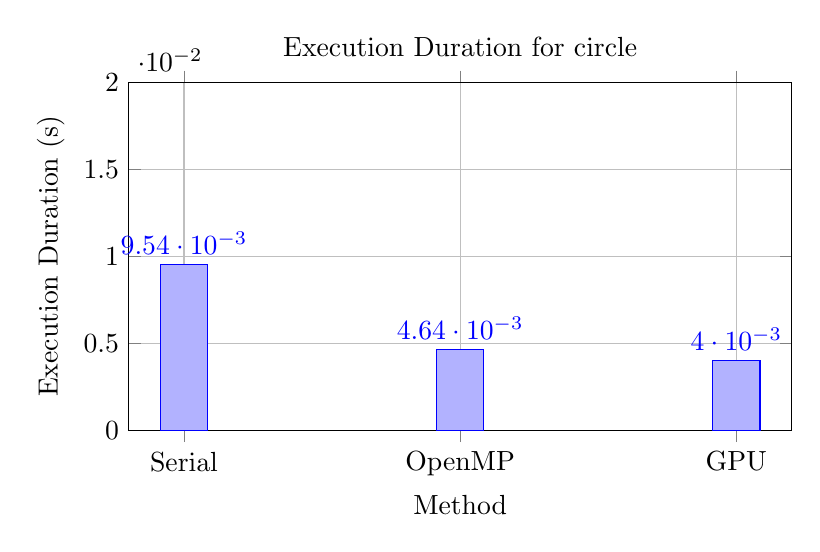
\begin{tikzpicture}
    \begin{axis}[
        ybar,
        bar width=.6cm,
        width=10cm,
        height=6cm,
        ylabel={Execution Duration (s)},
        xlabel={Method},
        symbolic x coords={Serial, OpenMP, GPU},
        xtick=data,
        nodes near coords,
        ymin=0, ymax=0.02,
        grid=major,
        title={Execution Duration for circle}
    ]
        \addplot coordinates {(Serial,0.00953500) (OpenMP,0.00463942) (GPU,0.00400282)};
    \end{axis}
\end{tikzpicture}
\caption{Comparison of execution duration for the dataset Circle: N4000 with different implementation methods. Experiments are conducted on an Intel i9-13980HX consumer CPU and NVIDIA RTX4070 consumer GPU with 512 threads per thread block}\label{fig:circle}
\end{figure}

\subsection{Hepta}
\begin{figure}[H]
\centering
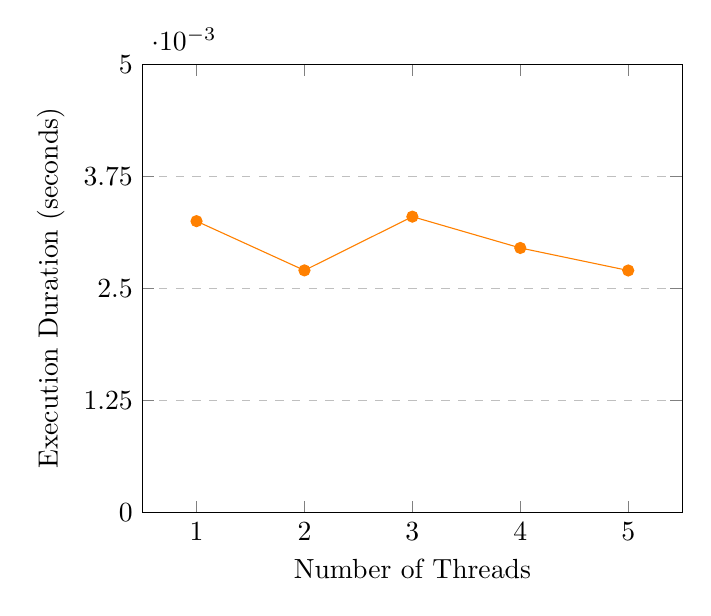
\begin{tikzpicture}
\begin{axis}[
    xlabel={Number of Threads},
    ylabel={Execution Duration (seconds)},
    xmin=0.5, xmax=5.5,
    ymin=0, ymax=0.005,
    xtick={1, 2, 3, 4, 5},
    ytick={0, 0.00125, 0.0025, 0.00375, 0.005},
    ymajorgrids=true,
    grid style=dashed,
]
\addplot[
    color=orange,
    mark=*,
    ]
    coordinates {
    (1,0.003249520) (2,0.002700380) (3,0.003299843) (4,0.002950533) (5,0.002699282)
    };

\end{axis}
\end{tikzpicture}
\caption{Execution Duration vs. Number of Threads for Hepta}
\label{fig:hepta}
\end{figure}

\subsection{Isolation}
% Isolation
\begin{figure}[H]
\centering
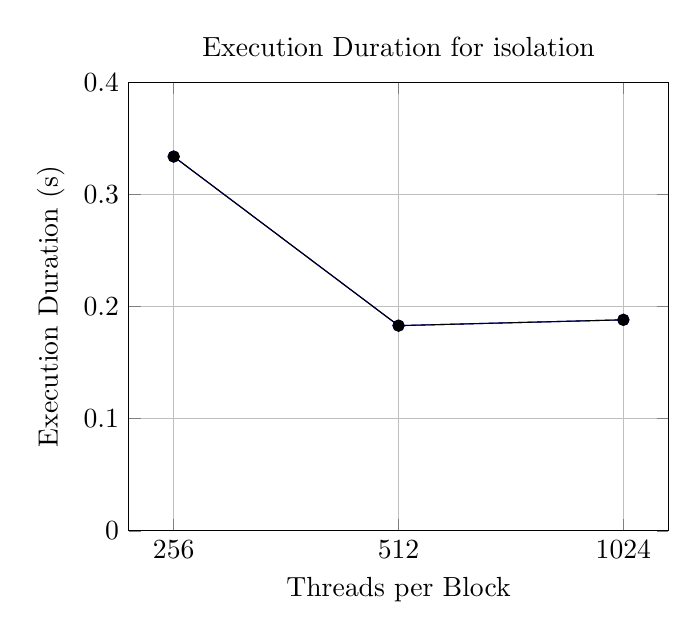
\begin{tikzpicture}
    \begin{axis}[
        xlabel={Threads per Block},
        ylabel={Execution Duration (s)},
        symbolic x coords={256, 512, 1024},
        xtick=data,
        ymin=0, ymax=0.4,
        grid=major,
        title={Execution Duration for isolation}
    ]
        \addplot coordinates {(256,0.333926) (512,0.183065) (1024,0.188247)};
        \addplot[mark=*] coordinates {(256,0.333926) (512,0.183065) (1024,0.188247)};
    \end{axis}
\end{tikzpicture}
\caption{Comparison of execution duration for the dataset Isolation: N9000 with different
threads per thread block. Experiments are conducted on an NVIDIA RTX4070 consumer GPU}
\end{figure}

\subsection{Smile}
\begin{figure}[H]
\centering
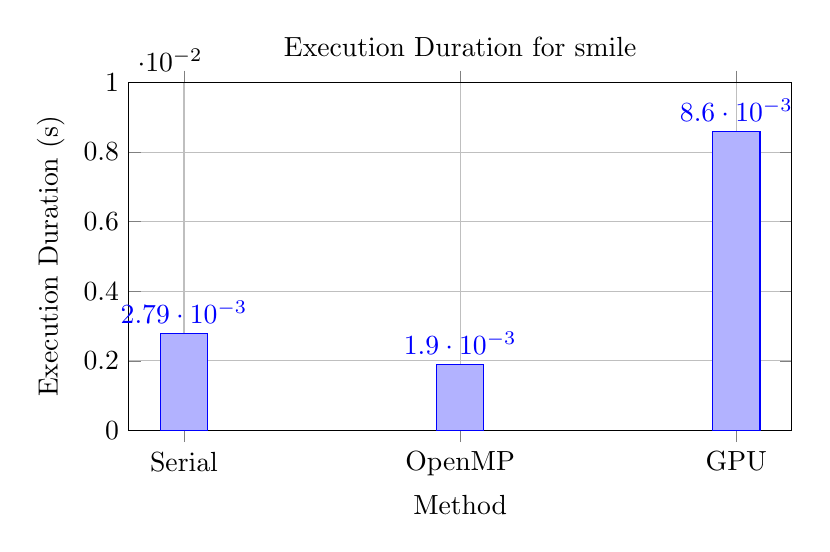
\begin{tikzpicture}
    \begin{axis}[
        ybar,
        bar width=.6cm,
        width=10cm,
        height=6cm,
        ylabel={Execution Duration (s)},
        xlabel={Method},
        symbolic x coords={Serial, OpenMP, GPU},
        xtick=data,
        nodes near coords,
        ymin=0, ymax=0.01,
        grid=major,
        title={Execution Duration for smile}
    ]
        \addplot coordinates {(Serial,0.00278600) (OpenMP,0.00190175) (GPU,0.00859648)};
    \end{axis}
\end{tikzpicture}
\caption{Comparison of execution duration for the dataset Circle: N1000 with different implementation methods. Experiments are conducted on an Intel i9-13980HX consumer CPU and NVIDIA RTX4070 consumer GPU with 512 threads per thread block}\label{fig:smile}
\end{figure}


We can see that number of increase in processors mostly results in decaying the execution time. But we can also see that in some cases there are fluctuations, not an absolute monotonic decaying behavior in each case.  This behavior can be observed in the figure \ref{fig:hepta}. It can be observed from the figure \ref{fig:birch} when the data points are relatively large, increasing the processor number results in a monotonic decaying execution duration. These behaviors can be explained using the Gustafson’s law.


